\chapter{Primeros pasos}
\setcounter{page}{4}

\section{Obteniendo la aplicaci\'on}
Para obtener una copia de la \'ultima versi\'on de la aplicaci\'on ingrese con
su dispositivo \blackberry a la direcci\'on \emph{http://www.ehmsoft.com/ota},
all\'i confirma la descarga y despu\'es tendr\'a una versi\'on
totalmente funcional de la aplicaci\'on en su versi\'on m\'ovil.
\section{Ingresando por primera vez}
La primera vez que ingrese se le presentar\'a un mensaje con la licencia de la
aplicaci\'on, despu\'es de aceptarla ver\'a un di\'alogo en el que
introducir\'a la clave del producto que se le otorg\'o, cuando esta ha sido
validada estar\'a en una pantalla con fondo oscuro, esta es la pantalla inicial
de la aplicaci\'on.
\footnote{En caso de problemas con su clave de producto env\'ie un correo
electr\'onico a \mbox{soporte@ehmsoft.com}}


\section{Cosas que debe saber}
La aplicaci\'on cuenta con ciertos elementos que le ayudar\'an a tener una
mejor experiencia con la aplicaci\'on. A continuaci\'on se explicar\'an cuales
son dichos elementos:

\subsection{Buscador en cada listado}
Cuando aprenda sobre los listados
(P\'ag.\pageref{sec:consultandoLaInformacion}) podr\'a ver que todos ellos tienen
un buscador por defecto,
\footnote{Este puede ser desactivado en las preferencias
(P\'ag.\pageref{sec:busquedaPantallas})}
 con este podr\'a realizar b\'usquedas en tiempo real de cada campo que puede
contener cada elemento del listado. Para iniciar la b\'usqueda solamente tiene
que empezar a digitar la palabra que quiere buscar en el teclado de su
dispositivo \blackberry.
\subsection{Plantillas}
Son elementos \'utiles cuando usted desea crear procesos con
caracter\'isticas similares de forma r\'apida. Una plantilla contiene los mismos
campos de un proceso y en base a esta podr\'a crear procesos con esos campos
pre-ingresados.
\subsection{Campos personalizados}
En sus procesos y plantillas podr\'a agregar campos personalizados, estos son
\'utiles cuando usted desea agregar informaci\'on extra a un proceso. Por
ejemplo: Nombre del juez.
\subsection{Pantalla inicial}
La primera pantalla que ve al iniciar la aplicaci\'on tiene como funci\'on
informar las actuaciones que tienen vencimiento pr\'oximo en orden
cronol\'ogico.
\footnote{La cantidad mostrada puede ser modificada en las preferencias
(P\'ag. \ref{sec:actuacionesCriticas})}
Debe tener presente que una actuaci\'on pudo haberse vencido hace horas y aun
as\'i ser listada, esto se debe a que se muestran con respecto al d\'ia y no a
la hora de vencimiento, esto para evitar posibles p\'erdidas de citas.

En el listado puede observar si su cada actuaci\'on tiene una cita por medio de
los s\'imbolos de una campana para saber si tiene cita y un reloj indica si
tiene alarma.

Al situarse sobre una actuaci\'on podr\'a verla (editarla) desplegando el
men\'u \blackberry y seleccionando \emph{Ver actuaci\'on}. Tambi\'en podr\'a
ver el proceso asociado a una actuaci\'on desplegando el men\'u \blackberry y
seleccionando \emph{Ver proceso} (Fig. \ref{fig:pantallaInicialMenu}).

\begin{figure}[htb]
\begin{center}
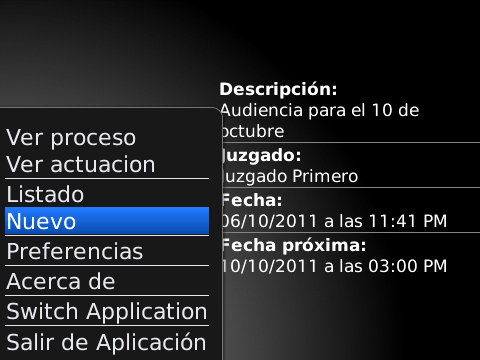
\includegraphics[scale=0.4]{./CapturasDePantalla/PantallaInicial/MenuPrincipal-Nuevo.png}
\caption{Men\'u en la pantalla inicial}\label{fig:pantallaInicialMenu}
\end{center}
\end{figure}